\documentclass{article}
\usepackage{graphicx} % new way of doing eps files
\usepackage{listings} % nice code layout
\usepackage[usenames]{color} % color
\definecolor{listinggray}{gray}{0.9}
\definecolor{graphgray}{gray}{0.7}
\definecolor{ans}{rgb}{1,0,0}
\definecolor{blue}{rgb}{0,0,1}
% \Verilog{title}{label}{file}
\graphicspath{ {H:/ELC3338/Team8/CompOrg_Spring2018_S1_Team8/images/} }
\newcommand{\Verilog}[3]{
  \lstset{language=Verilog}
  \lstset{backgroundcolor=\color{listinggray},rulecolor=\color{blue}}
  \lstset{linewidth=\textwidth}
  \lstset{commentstyle=\textit, stringstyle=\upshape,showspaces=false}
  \lstset{frame=tb}
  \lstinputlisting[caption={#1},label={#2}]{#3}
}


\author{Breana Leal and Matthew Carrano}
\title{Lab 9 - iExecute and Datapath}

\begin{document}
\maketitle

\section{Introduction}
The goal of this lab is completing the iExecute stage and integrating the iExecute stage into the overall datapath. Once constructed, the outputs are verified through simulation and an expected results table.

\section{Interface}
The iExecute module has inputs pc\_in, read\_data1, read\_data2, sign\_extended\_output, alu\_op, opcode, and alu\_src. It has outputs branch\_target, alu\_result, and zero. The next five modules are part of the iExecute module. 

The inputs of the mux are read\_data2 and sign\_extended\_output. The control signal is alu\_src, this signal chooses which of the two above signals to output. The output is mux\_out.  
The shifter module left shifts the bits of its input, sign\_extended\_out, and outputs shift\_result. 
The inputs of the adder module are pc\_in and shift\_result. These two values are added and the result, and therefore output, is branch\_target.
The alu\_control module inputs are alu\_op and opcode. The output is control.
The ALU module has inputs read\_data1, mux\_out, and control. The outputs are alu\_result and zero. 
The final module is the ALU. This module has inputs control, read\_data1, and mux\_out. It's outputs are alu\_result and zero. 

\section{Design}
iExecute is one unit with five internal modules. The modules are shifter (alu\_shifter), mux (alu\_mux), adder (branch\_adder),alu\_control (ex\_alu\_con), and ALU (ex\_alu ). The following process applies to instructions with branch addressing. The iExecute uses the adder and shifter to left shift the sign extended address add the address with the current PC to provide the execute's branch target. Additionally, it uses the ALU control to determine the operations of the ALU. The ALU does arithmetic operations on its inputs and outputs the results as well as a flag which is 1 when the result is 0 and 0 otherwise. Overall, iExecute provides the current branch targeted address, a zero flag, and ALU operation results.

The datapath.v links the iExecute, iDecode, and iFetch modules. As described previously, the iDecode stage will process the outputted instruction from the Fetch stage. Similarly, iExecute engages the read\_data1, read\_data2, and iDecode's extended address target to output the current branch target address, ALU result, and zero flag.

\section{Implementation}
The following modules are part of the iExecute module.

The mux module is implemented using the ? operator. If the control signal is 0, mux\_out is set to a\_in. If the control signal is 1, mux\_out is set to b\_in. In the iExecute module, signals read\_data2, sign\_extended\_output, alu\_src, and mux\_out, correspond to signals a\_in, b\_in, control, and mux\_out of the mux module, respectively. In this way the control module from the iDecode stage can control which signal goes to the ALU module. The code can be found in Listing~\ref{code:mux} on page~\pageref{code:mux}.

The shifter module is implemented by left shifting the input (offset) by 2 using the  \textless\textless\space operator and assigning the result to "result". This is done inside an always@(*) block (sequential logic) and therefore a non-blocking assignment is used. In this way the result is set at any change to offset. In the iExecute module, signals sign\_extended\_output and shift\_result, correspond to signals offset and result of the shifter module, respectively. The code can be found in Listing~\ref{code:shifter} on page~\pageref{code:shifter}.

The adder module is implemented using the + operator to add the inputs a\_in and b\_in. The result is assigned to add\_out using a continuous assignment. In the iExecute module, signals pc\_in, shift\_result, and branch\_target, correspond to signals a\_in, b\_in, and add\_out of the adder module, respectively. In this configuration the adder outputs the next address of the program counter by adding the current pc with the left shifted sign extended address. The code can be found in Listing~\ref{code:adder} on page~\pageref{code:adder}. 

The alu\_control module was implemented using a case statement inside of an always@(*) block. The case statement is constructed using the alu\_op signal as the switch variable and macros for the possible values of alu\_op as the cases. Each case sets the control\_bits to a specific 4-bit value using a non-blocking assignment. These values will control the operation of the ALU. The default case is the d-type control signal because this is a fast ALU operation. Because of the always block, the control\_bits signal will be set with any change to alu\_op or opcode. In the iExecute module the signals are named the same except control in corresponds to control\_bits in the alu\_control module. The code can be found in Listing~\ref{code:alucontrol} on page~\pageref{code:alucontrol}.

Like the alu\_control module, the ALU module is implemented using a case statement inside of an always@(*) module. The case statement is constructed with control as the switch variable, and the control signals from the alu\_control module as the cases. The result signal is set in each of the case blocks using a non-blocking assignment. If the control signal is signal for an add instruction, the result is the sum of data\_1 and data\_2. If the control signal is the signal for a conditional branch, the result is set to data\_2. The rest of the cases can be seen in Listing~\ref{code:ALU} on page~\pageref{code:ALU}. Lastly, the flag output signal is set to the result of the Boolean logic statement, (result==0). This means that flag is 1 if the result is 0, and 0 if the result is not 0. With this module the datapath can do the necessary mathematical operations on all of its signals. The code can be found in Listing~\ref{code:ALU} on page~\pageref{code:ALU}.    

The iExecute module was implemented simply by instantiating each of the five modules above and connecting them as described above. This can be seen further in Listing~\ref{code:iExecute} on page~\pageref{code:iExecute}. This module completes the execute stage of the processor.   

\Verilog{Verilog code for implementing the mux.}{code:mux}{../code/0_common/mux.v}
\Verilog{Verilog code for implementing the adder.}{code:adder}{../code/1_fetch/adder.v}
\Verilog{Verilog code for implementing the shifter.}{code:shifter}{../code/3_execute/shifter.v}
\Verilog{Verilog code for implementing the ALU control.}{code:alucontrol}{../code/3_execute/alu_control.v}
\Verilog{Verilog code for implementing the ALU.}{code:ALU}{../code/3_execute/ALU.v}
\Verilog{Verilog code for implementing the iExecute module.}{code:iExecute}{../code/3_execute/iExecute.v}

\section{Test Bench Design}
The iExecute test bench creates regs for all inputs and wires for all outputs. Zero and alu\_src are 1 bit, alu\_op is 2 bits, opcode is 11 bits, and all other signals are 64 bits. An iExecute module is instantiated. Values are set in the initial section every cycle (10ns). In the first cycle a value is set for all inputs. 

The iExecute test bench underwent 14 operations each requiring either subtraction, addition, bit-wise OR, load, store, CBZ comparison, or branching operations. Before testing, our definitions included each operation as a separate macro for its specific instruction and instruction type. Each instruction has 11 bits, CBZ and B have non-applicable Xs for unnecessary bits. The three defined types, R-type, D-type, and Branch are two bit macros. Figure 1 demonstrates the header changes. The initial values for read\_data1 and read\_2 are 10 and 15. They are redefined after the ninth, twelfth, and thirteenth cycle to 15 and 15, 15 and 0, 15 and 15 respectively (since there is no write data signal). The connecting wires are associated with its three external pieces, branch target, zero, and ALU result.


\Verilog{Verilog code for testing the Execute stage.}{code:mux}{../code/3_execute/iExecute.v}
\begin{figure}[h]	
	\caption{Updated Definitions Header.}
	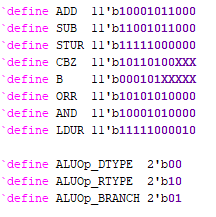
\includegraphics{Macros_lab9}
	\label{fig:macros}
	\centering
\end{figure}
Datapath is the top hierarchy testbench for debugging and connecting stages together. iExecute is an additional stage to bridge towards a single completed ARM datapath. With the iExecute module implemented it now only needs initial values to start the program counter, as well as write\_data values to store alu results in the correct registers. 

\Verilog{Verilog code for testing the Updated Datapath.}{code:mux}{../code/2_decode/datapath.v}


\section{Simulation}
The timing diagrams in Figure 2 and 3 verify that iExecute stage is functioning properly within the datapath and has outputs corresponding to our expected results table Figure 4.
\begin{figure}[h]	
	\caption{Timing diagram for iExecute module test.}
	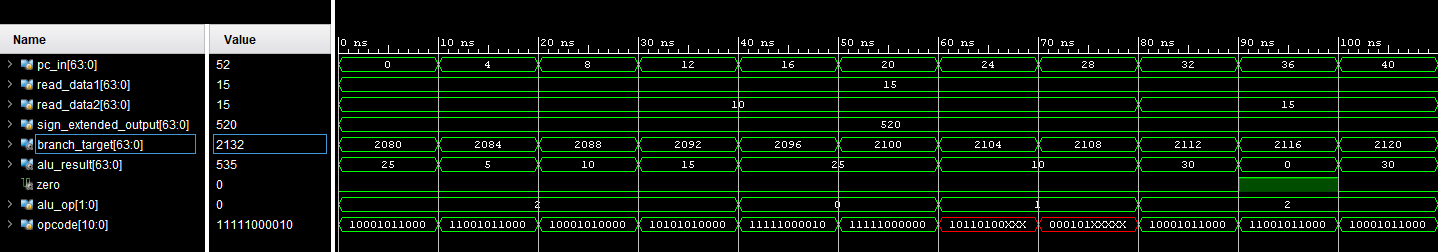
\includegraphics[width=\textwidth]{iExecute_Sim}
	\label{fig:iExecutesim}
	\caption{Timing diagram for datapath module test.}
	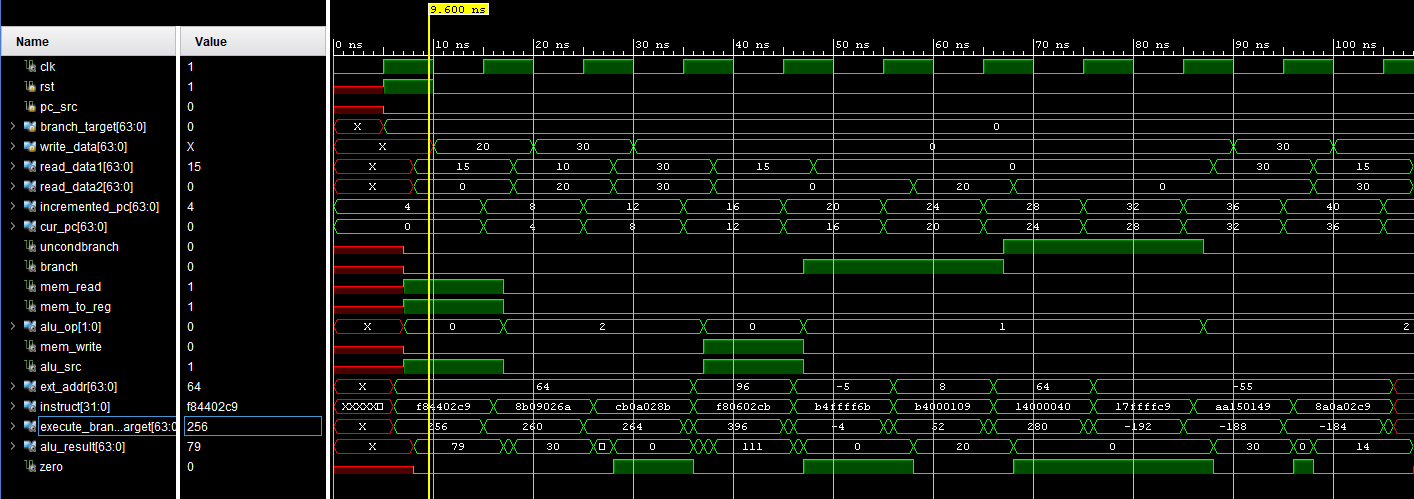
\includegraphics[width=\textwidth]{datapath_with_execute}
	\label{fig:datapathsim}
	\caption{Expected Results Table.}
	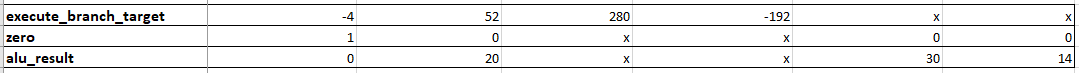
\includegraphics[width=\textwidth]{Expected_results_table_EXECUTE}
	\label{fig:expectedresults}
\end{figure}



\section{Conclusions}
The iExecute module and datapath testbench were created and updated. iExecute is our third stage that provides an updated brancg target, ALU results, and zero flag. Its input are the iDecode's wire connecting outputs. The iFetch, iDecode, and iExecute are linked in the datapath testbench. The testbench demonstrates the ARM's increments fetched at proper times and providing correctly executed results.

\end{document} 